\documentclass{beamer}

\usetheme{focus} 
\definecolor{main}{RGB}{92, 138, 168}
\definecolor{background}{RGB}{240, 247, 255}

\usepackage[spanish]{babel}
\usepackage{amsmath, amsthm, amssymb}
%----------------------------------------------------------------------------------------
%	 TITLE SLIDE
%----------------------------------------------------------------------------------------

\title{Moogle!: \\ Document Search Engine}

\author{Jocdan L. López Mantecón}

\titlegraphic{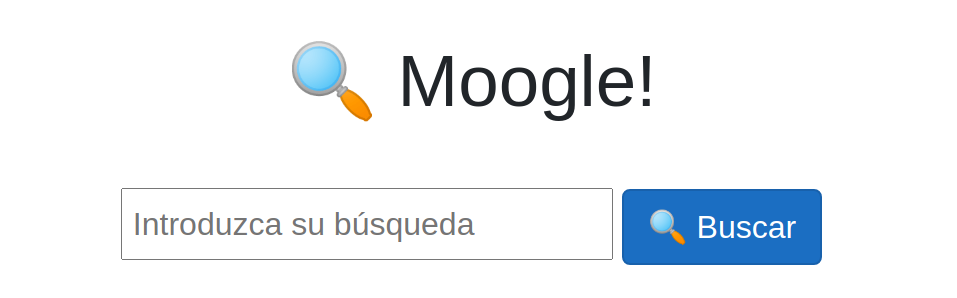
\includegraphics[scale=1.25]{Images/moogle.png}

\institute{Facultad de Matemática y Computación\\Universidad de la Habana}

\date{Julio 2023}

%------------------------------------------------

\begin{document}

%------------------------------------------------

\begin{frame}
	\maketitle 
\end{frame}

%----------------------------------------------------------------------------------------
%	 SECTION 1
%----------------------------------------------------------------------------------------

\section{Que es Moogle!?}\label{intro}

%------------------------------------------------

\begin{frame}
	Moogle! es una aplicación *totalmente original* cuyo propósito es buscar inteligentemente un texto en un conjunto de documentos, es decir un motor de búsqueda de documentos de archivos txt basándose en el Modelo del Espacio Vectorial para la Recuperación de Información.
	
	\pause
	
	Es una aplicación web, desarrollada con tecnología .NET Core 7.0, específicamente usando Blazor como *framework* web para la interfaz gráfica, y en el lenguaje C#.
	La aplicación está dividida en dos componentes fundamentales:
	
	- \textbf{MoogleServer} es un servidor web que renderiza la interfaz gráfica y sirve los resultados.
	- \textbf{MoogleEngine} es una biblioteca de clases donde está implementada la lógica del algoritmo de búsqueda.
\end{frame}

\section{Fundamentos Teóricos}\label{fundamentals}

\begin{frame}{Modelo de Espacio Vectorial para la Recuperación de Información (MEV)}
	 \begin{itemize}
		\item Consiste en representar los documentos como vectores de las palabras que los
		constituyen.
		\pause
		\item Se construye un vocabulario con todas las palabras de la colección de documentos
		de forma que no se repitan los términos y cada uno de estos términos representa una dimensión
		del espacio.
		\pause
		\item La query se trata como un pseudo-documento y se representa mediante un vector en el espacio. 
		\pause
		\item Se emplean indicadores de similitud para determinar que documentos son similares a otros o a una
		query dada.
	\end{itemize}
\end{frame}

\begin{frame}{Term Frequency Inverse Document Frequency (TF-IDF)}
	\begin{itemize}
		\item \emph{Frecuencia de términos (TF):} mide la frecuencia relativa con la que un término aparece
		en un documento, es decir, cuantas veces aparece el término en el documento
		(frecuencia absoluta Nw) dividido por la cantidad total (Td) de palabras del documento. La
		fórmula utilizada es:
		
		\begin{center}    
			\begin{equation}
				TF_w = \frac{N_w}{T_d}
			\end{equation}
		\end{center}
		La intuición con esta medida es que los términos que aparecen más veces
		probablemente sean más importantes para el contenido del documento.
		
		\pause
		\item \emph{Frecuencia inversa de documento (IDF):} Mide la importancia del término en la colección
		de documentos, es decir, cuantos documentos de la colección contienen el término.
		Se empleó la fórmula:
		\begin{center}
			\begin{equation}
				IDF_w = \log_2(\frac{|D|}{|d_w|})   
			\end{equation}
		\end{center}
		La idea que subyace esta medida es que los términos que aparecen en muchos
		documentos probablemente sean menos importantes y los que aparecen en menos
		documentos son más específicos y más relevantes para la búsqueda
		
		\pause
		\item La medida TF-IDF asigna un peso a cada término en cada documento de la colección. El peso
		de un término se calcula multiplicando la frecuencia del término TF por la frecuencia inversa del
		documento IDF:
		\begin{center}
			\begin{equation}
				weight = TF_w * IDF_w 
			\end{equation}
		\end{center}
		
	\end{itemize}
	
\end{frame}

\begin{frame}{Similitud de Cosenos}
	
		Compara la similitud entre dos vectores, segun el ángulo entre los mismos
		\pause
		\begin{center}
			\begin{equation}
				sim(A, B) = \frac{\overrightarrow{A} * \overrightarrow{B}}{||A|| * ||B||} 
			\end{equation}
		\end{center}
		\pause
		\begin{center}
			\begin{equation}
				\overrightarrow{A} * \overrightarrow{B} = \Sigma(a_i * b_i)
				\tag*{Producto Vectorial}
			\end{equation}
		\end{center}
		\pause
		\begin{center}
			\begin{equation}
				\tag{Norma de un vector}
				||A|| = \sqrt{\Sigma a_i^2}
			\end{equation}
		\end{center}.
	
\end{frame}

\section{Utilidades}\label{utilites}
\begin{frame}{Generando el snippet:}
	Para generar del snippet se decidió mostrar un subtexto del documento que contenga la palabra
	de la query de mayor importancia (mayor TF-IDF). b Se extrae inicialmente un snippet con un
	tamaño de 80 caracteres alrededor de la palabra mas importante de la query con respecto al
	documento y al corpus; a partir de este primer resultado seguimos tomando caracteres hasta
	llegar al comienzo y al final de la oración completa respectivamente buscando la primera
	aparición de los signos de puntuación más comunes que pueden delimitar una oración: “ ¿? .
	; ¡! ”
\end{frame}

\begin{frame}{Generando el snippet:}
\begin{itemize}
	\item Se emplea la Distancia de Edición o Distancia de Levenshtein. 
	La Distancia de Levenshtein o distancia de Edición es una medida de que tan similares son dos
	strings. Se define como el mínimo número de transformaciones (insertar, eliminar o remplazar)
	que se necesitan para convertir uno de los strings en el otro.
	\pause
	\item Si alguna palabra de la query no aparece en el vocabulario del corpus y no es una
	stopword entonces se calcula la distancia de edición entre dicha palabra y todos los términos
	del vocabulario y sustituimos esta con la palabra del vocabulario con menor distancia de edición.
	Luego se sustituye esta palabra en la query.
\end{itemize}
\end{frame}

\begin{frame}{Operadores de Busqueda}
Se implementaron cuatro operadores de búsqueda:
	\begin{itemize}
	\item  Existe $\wedge$ : Las palabras a la que se aplica a este operador debe aparecer en los
	documentos que se muestran como resultados de la busqueda. Si el documento a
	evaluar no contine la palabra operando (a las cuales se denominaron markers) se
	disminuye su score en un 100$\%$ , en caso contrario permanece inalterado:
	
	\item NoExiste ! : Los marcadores de este operador no deben aparecer en los resultados de
	búsqueda. Si el documento contiene dicho marcador disminuye su score en 100\% en
	caso contrario permanece inalterado:
	
	\item Importancia *: Este operador se puede emplear N veces consecutivas al inicio de la
	palabra. Por cada vez que se utilice se incrementa el score del documento que contenga
	los marcadores de este operador en un 35\%.
	\end{itemize} 
\end{frame}
			
\begin{frame}{Operadores de Busqueda}
	Distancia~: Operador binario la	distancia entre dos palabras dadas incrementa el score del documento de forma tal que a menor
	distancia mayor es el incremento. 
	
	\begin{center}
		La función que caracteriza este operador es:
		
		\begin{equation}
			~mod = 1.00 - \frac{dist(w_1,w_2)}{doc.Length}
		\end{equation}
	\end{center}
	Donde $dist(w_1, w_2)$ es la menor distancia entre las dos palabras en el
	documento y doc.Lenght es la cantidad total de caracteres del documento.
	De esta forma, si la distancia entre las palabras es pequeña entonces el segundo término
	de la expresión tiende a cero y el factor tiende a 1.00 (100\%); de lo contrario, si la
	distancia es grande entonces el segundo término tiende a 1 y el factor tiende a 0%.
\end{frame}



\end{document}
